\subsubsection{Benchmark for chunk size}

To transfer a message from a source to a destination through intermediate nodes, we split the message into smaller chunks and keep sending the chunks into the network. This is to reduce the waiting time at the intermediate nodes, thus, reduce total transfer time. We carried out an experiment to show optimal chunk sizes for different message sizes. In this experiment, we varied the message sizes from 8 KB up to 8 MB. The chunk sizes also varied from 4KB up to 1MB. The experiment is carried out in 512-node partition using subset pattern in which first 32 nodes send data to last 256 nodes. The results are shown in Figure \ref{fig:chunksize}.

\begin{figure}[!htb]
\vspace{-0.1in}
\centering
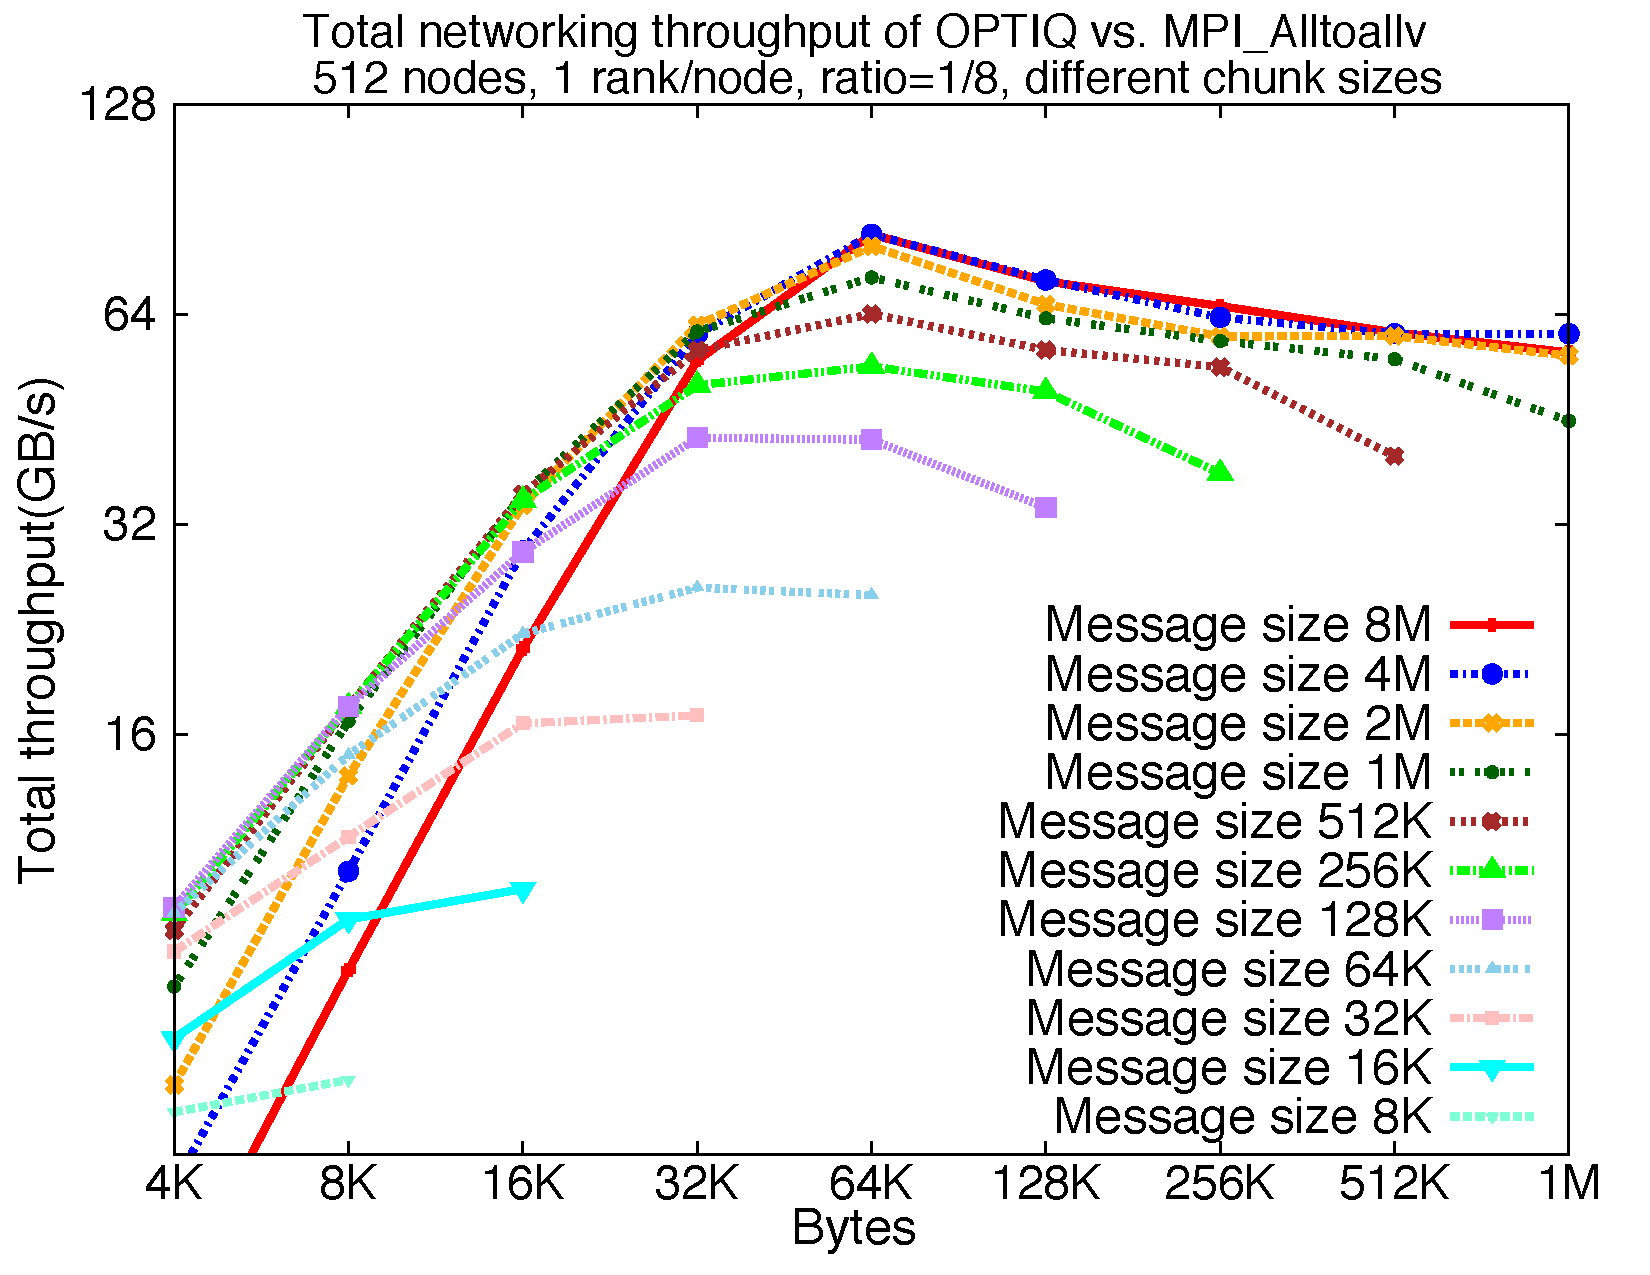
\includegraphics[scale=0.30]{figures/87_chunksize.pdf}
\vspace{-0.1in}
\caption{Chunk sizes and their performance in 512-node partition, subset pattern.}
\vspace{-0.1in}
\label{fig:chunksize}
\end{figure}

As shown in the Figure \ref{fig:chunksize}, for messages with sizes less than 16 KB, we should transfer the entire mesasges. With message size 32 KB, we can use chunksize 16 KB. With message sizes 64 KB or 128 KB, we can use 32 KB chunksize. With larger message sizes, we can use 64 KB chunk size. Similar trends are found in disjoint and overlap patterns. For the expriments in this paper, we use 64 KB chunk size.

